\documentclass[border=6pt]{standalone}
\usepackage[T1]{fontenc}
\usepackage{lmodern}
\usepackage{amsmath}
\usepackage{tikz}
\usetikzlibrary{arrows.meta,positioning,calc}
\definecolor{swinc}{HTML}{2166AC}
\definecolor{cnnc}{HTML}{1B7837}
\definecolor{decc}{HTML}{E66101}
\newcommand{\code}[1]{\texttt{\detokenize{#1}}}
\begin{document}
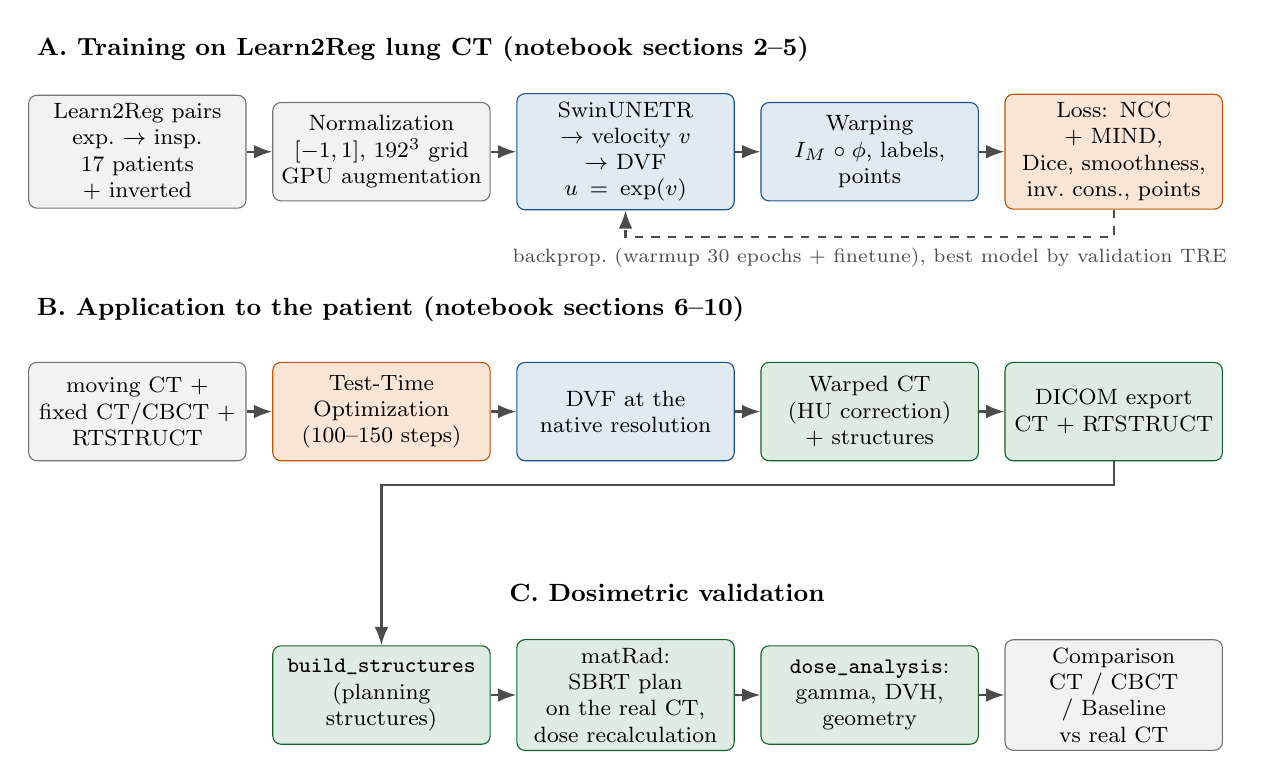
\begin{tikzpicture}[
  font=\footnotesize, >=Latex,
  st/.style={draw, rounded corners=3pt, align=center, minimum height=1.25cm, text width=2.55cm, inner sep=3pt},
  dat/.style={st, fill=black!5, draw=black!55},
  net/.style={st, fill=swinc!14, draw=swinc!80!black},
  opt/.style={st, fill=decc!16, draw=decc!85!black},
  clin/.style={st, fill=cnnc!14, draw=cnnc!80!black},
  arr/.style={->, thick, black!70}
]
\node[font=\small\bfseries, anchor=west] at (-1.4,1.3) {A. Training on Learn2Reg lung CT (notebook sections 2--5)};
\node[dat] (d1) at (0,0) {Learn2Reg pairs\\ exp.\ $\to$ insp.\\ 17 patients + inverted};
\node[dat] (d2) at (3.1,0) {Normalization\\ $[-1,1]$, $192^3$ grid\\ GPU augmentation};
\node[net] (d3) at (6.2,0) {SwinUNETR\\ $\to$ velocity $v$\\ $\to$ DVF $u=\exp(v)$};
\node[net] (d4) at (9.3,0) {Warping\\ $I_M\circ\phi$, labels,\\ points};
\node[opt] (d5) at (12.4,0) {Loss: NCC + MIND,\\ Dice, smoothness,\\ inv.\ cons., points};
\draw[arr] (d1) -- (d2); \draw[arr] (d2) -- (d3); \draw[arr] (d3) -- (d4); \draw[arr] (d4) -- (d5);
\draw[arr, dashed] (d5.south) -- ++(0,-0.35) -| node[pos=0.25, below, font=\scriptsize] {backprop.\ (warmup 30 epochs + finetune), best model by validation TRE} (d3.south);

\begin{scope}[yshift=-3.3cm]
\node[font=\small\bfseries, anchor=west] at (-1.4,1.3) {B. Application to the patient (notebook sections 6--10)};
\node[dat] (t1) at (0,0) {moving CT +\\ fixed CT/CBCT +\\ RTSTRUCT};
\node[opt] (t2) at (3.1,0) {Test-Time\\ Optimization\\ (100--150 steps)};
\node[net] (t3) at (6.2,0) {DVF at the\\ native resolution};
\node[clin] (t4) at (9.3,0) {Warped CT\\ (HU correction)\\ + structures};
\node[clin] (t5) at (12.4,0) {DICOM export\\ CT + RTSTRUCT};
\draw[arr] (t1) -- (t2); \draw[arr] (t2) -- (t3); \draw[arr] (t3) -- (t4); \draw[arr] (t4) -- (t5);
\end{scope}

\begin{scope}[yshift=-6.9cm]
\node[font=\small\bfseries, anchor=west] at (4.6,1.3) {C. Dosimetric validation};
\node[clin] (c1) at (3.1,0) {\code{build_structures}\\ (planning\\ structures)};
\node[clin] (c2) at (6.2,0) {matRad: SBRT plan\\ on the real CT,\\ dose recalculation};
\node[clin] (c3) at (9.3,0) {\code{dose_analysis}:\\ gamma, DVH,\\ geometry};
\node[dat] (c4) at (12.4,0) {Comparison\\ CT / CBCT / Baseline\\ vs real CT};
\draw[arr] (c1) -- (c2); \draw[arr] (c2) -- (c3); \draw[arr] (c3) -- (c4);
\end{scope}
\draw[arr] (t5.south) -- ++(0,-0.3) -| (c1.north);
\end{tikzpicture}
\end{document}
